\documentclass[acmsmall, nonacm]{acmart}

\usepackage[utf8]{inputenc} % allow utf-8 input
\usepackage[T1]{fontenc}    % use 8-bit T1 fonts
\usepackage{hyperref}       % hyperlinks
\usepackage{url}            % simple URL typesetting
\usepackage{booktabs}       % professional-quality tables
\usepackage{amsfonts}       % blackboard math symbols
\usepackage{nicefrac}       % compact symbols for 1/2, etc.
\usepackage{microtype}      % microtypography

\usepackage{amsmath,amssymb}
\usepackage{graphicx,grffile}

\usepackage{longtable}
\usepackage{subcaption}
\usepackage{xcolor}


\title{State description language and PathRL}

% XXX contributors' macros
% gleb
\newcommand{\GG}[1]{\textcolor{red}{[GG: #1]}}
% daniil
\newcommand{\danil}[1]{{\color{red} [#1]}}
% ivan
\newcommand{\attn}[1]{{\color{magenta}{\textbf{#1}}}}


\begin{document}

\maketitle

\section{PathRL algorithm}

\subsection{Definitions}

An MDP is a tuple $(\mathcal{S}, \mathcal{A}, \mathcal{P}, \mathcal{R}, \gamma)$. An observation lies in space $\mathcal{O}$ and is denoted by $O_i$. An inner representation of an observation is denote by $h_i \in \mathcal{H}$. We call a \emph{hash} \attn{representation} function $
f: \mathcal{O} \rightarrow \mathcal{H}
$. We suppose that the goal agent ``talks'' with the navigation agent via a sequence of messages expressed as points in $\mathcal{H}$. All of works 

\begin{figure}
  \centering
  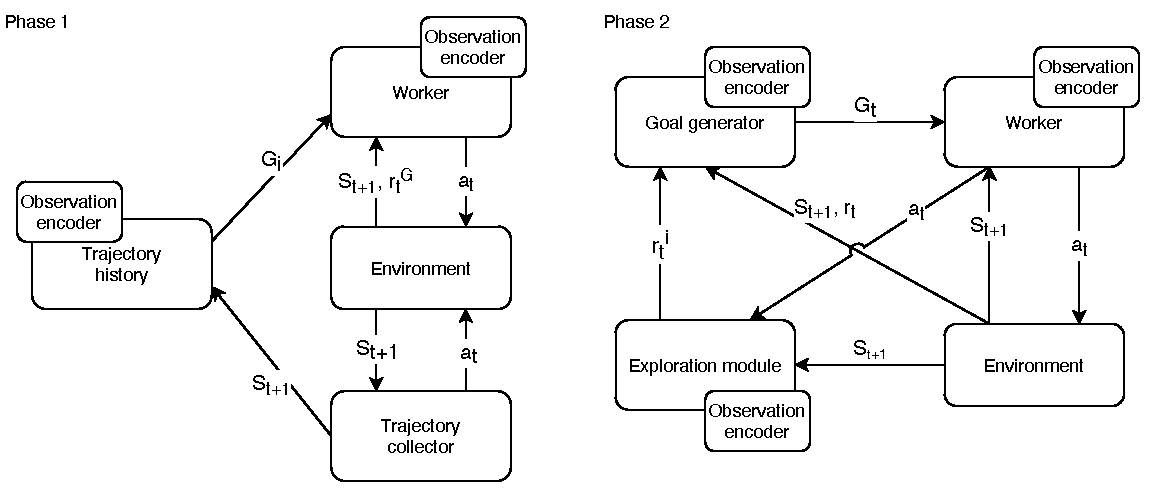
\includegraphics[width=0.9\linewidth]{./assets/diagram.pdf}
  \caption{PathRL alogorithm}
  \label{fig:pathrl}
\end{figure}

\subsection{First phase}


% XXX 1st phase: we just train a navigator using go-explore with HER and curiosity-driven third part explorer
The first phase of training can be described as a two-agent interaction: the encoder agent $E$ learns to produce a description of the task in some restricted inter-agent \emph{language}, and the navigator agent $N$ receives the task description and learns to execute it.
%
The \emph{language} can be similar to a query language wherein the desired state is described in a declarative form of instructions or predicates. The \emph{task} is a pair of queries which specify the initial states and the goals to be reached.
% XXX not just the abstract controllable embedding of target state, but its high level description, generated based on it (rich abstract state embedding). Besdies embedding is likely to be a compressed representation, which makes it unlikely to be a one-to-one mapping on $S$.
%
Both agents are rewarded if the navigator successfully executes the task, i.e. $N$ reaches the a goal set by $E$.
% In current work we consider only the singleton sets of states, hence, the task is defined as a pair of states.
This two-agent game is somewhat similar to the cooperative game proposed by~\citet{Mordatch2018EmergenceOG}.

Formally, the encoder $E$ takes is the desired state $s_g$ and produces its description $E(s_g)$, while the navigator $N$ reacts to this description and the current state $s_t$ by outputting the next action $a_t \sim N(s_t, E(s_g))$. Agent $E$ has no access to the current state $s_t$, which $N$ is in in the environment, and is thus forced to produce some declarative description of the desired state $s_g$, since it cannot communicate the exact sequence of actions $N$ has to perform.
% XXX maybe the target query and a hint vector? as it seems possible that the worker-agent could stray arbitrarily far away from the destination on the embedded state manifold

\subsubsection{Collecting the navigation tasks by exploration}

% the dataset resembles the go-explore-like replay buffer
Training an efficient navigator $N$ requires a diverse dataset of tasks $(s_t, s_g)$, in which a meaningful goal $s_g$ is attainable from an initial state $s_t$. To this end during training \emph{a third agent} randomly traverses the environment using some exploration policy $\mu_e$, thereby generating state-action trajectories that can be mined for feasible training tasks. The policy $\mu_e$ has to meet several requirements: it has to explore the environment reasonably well and the trajectories it produces must be diverse. One of the options is to use curiosity-based exploration \citep{pathak_curiosity-driven_2017,burda_exploration_2019}.

\subsubsection{Navigation reward}
\label{ssub:navigation_reward}

One possible training scheme is to shape the reward so that it encourages moving closer from the current state $s_t$ to the target state $s_g$. The notion of state \emph{proximity} must take into account the fact that states reside on certain latent manifold, must be consistent with respect to environment's randomness, and at the same time focus on controllable and abstract away uncontrollable or irrelevant features of the states. For example, positively rewarding for diminishing Euclidean distance between $s_g$ and $s_t$ fails all these desirable properties.

Specifically, in Random Disco Maze navigation environment, \citep{badia_never_2020}, the pixel-wise distance would hinder the task completion due to irrelevant random color of the labyrinth's walls. In the same environment the initial and goal states that are separated by an adjacent wall, yet unreachable from one another would be considered close states. Finally, in Pac-Man%
\footnote{
    \url{https://en.wikipedia.org/wiki/Pac-Man_(Atari_2600)}
}
the position of the player within the maze is a controllable feature, while the positions of patrolling ghosts are not, yet the distance between states would be sizeable, even if the protagonist has arrived exactly at the specified target position.
%
Similarly with Freeway%
\footnote{
    \url{https://en.wikipedia.org/wiki/Freeway_(video_game)}
}, the player's car is controllable, while the opponents' cars are not, \citep[fig.~1]{choi_contingency-aware_2019}.

% Another scheme is to reward agent from reaching the state that is similar enough to the target state. In this case, the state similarity function is not required to be transitive.

One possibility is to define a proximity score as $
    d(s_a, s_b) 
        := \frac{\phi(s_a)^\top \phi(s_b)}{\|\phi(s_a)\|\|\phi(s_b)\|}
$ -- the cosine similarity between the latent representations of states. The mapping $
    \phi \colon \mathcal{S} \to \mathbb{R}^{d_h}
$ is a learnt state embedding that removes features irrelevant to the navigator's task and effectively flattens the state manifold. The embedding $\phi$, that drops uncontrollable features can be trained in self-supervised manner on the inverse dynamics task. i.e. inferring the action taken between consecutive states, \citep{choi_contingency-aware_2019,badia_never_2020}.

% In this case the function $d(s_a, s_b)$ that estimates the similarity between states is required. The state similarity function should also be transitive i. e. if $d(s_a, s_b) > d(s_a, s_c)$ then $d(s_b, s_c) > d(s_a, s_c)$.
% XXX transitivity is $a \to b$, $b \to c$ implies $a \to c$.
% XXX the property above fails for euclidean distance: take an acute isosceles triangle.

\subsection{Second phase}

The second phase of training of this model is the addition of goal-setting agent $G$ which replaces encoder agent $E$ after training.
% XXX a fourth agent? Wasn't the encoder agent also the goal-setter in the beginning of this section?
% We should emphasize that our methodological contrib is the two-phased training (have to verify this)
%
This goal-setter receives only the current state and produces the set of predicates $e_g = G(s_t)$ that lead to potentially high rewards, i.e. $G$ learns to generate the set of predicates that describe high-reward states. During this phase actions are produced by pre-trained navigator $a_t = N(s_t, G(s_t))$ with frozen parameters, yet differentiable w.r.t. the goal-state embedding. This forces the goal agent $G$ to reproduce and communicate in the same description ``language'' as the encoder agent.


\subsubsection{Reward scheme}

The goal-setter $G$ is trained with two rewards: the extrinsic reward, i.e. true reward of the environment, and the intrinsic curiosity reward\textbf{} for active exploration.

In this scheme $G$ is encouraged to propose queries for states of two kinds: \emph{explotable} states with high extrinsic reward, and \emph{explorable}, unknown ``terrritory'' states high curiosity potential.
%
The combination of curiosity reward scheme and navigator agent have some parallels with Go-explore algorithm~\citep{ecoffet_first_2021}, where the navigation is done via virtual environment resets.


\subsection{World state representations}

The most promising possibility, especially in the context of the desiderata outlined in sec.~\ref{ssub:navigation_reward}, is to use compressed abstracted representations of the environment states in the encoder, the navigator and the goal-setting agents. The state internal embeddings produced by a world model pre-trained by the next state prediction task, \citep{ha_recurrent_2018}, or by an inverse dynamics model, \citep{badia_never_2020}.


\subsection{Motivation}

% XXX oof, i will reword this later.
The proposed scheme should be effective in sparse extrinsic reward settings: the low-level basic interaction in the environment, when trained to solve the environment on its own, would experience the detrimental effects of reward sparsity most acutely. However, if instead we train a low level agent on state-navigation tasks, motivating it for achieving the goals (a sort of synthetic intrinsic reward, but not curiosity-based), and delegate the solution of the environment itself to an abstract planning agent, which collects extrinsic rewards, we could effectively significantly reduce the planer's reward sparsity, since its consecutive states and actions are the milestones it sets for itself.

By splitting in two phases we are able to learn efficient reliable navigation skills using synthetic navigation tasks, 
without any extrinsic reward.
%
The proposed two-phase scheme should be effective for the multi-task learning setting in the same environment: a well trained and capable navigator model, even though trained for one specific environment and goal state distribution, can be effectively reused across different tasks.

As shown by \citet{ecoffet_first_2021} the exploration of distant states greatly improves the algorithm effectiveness. The availability of navigator agent enables training a goal agent, which is encouraged to explore remote states.
%
% XXX i am afraid this contribution is more of \citet{badia_never_2020,choi_contingency-aware_2019} rather than ours.
In contrast to \citep{ecoffet_first_2021}, though, by using learnt state representations that abstract away irrelevant information, and by decoupling goal-setting from goal-achieving the scheme proposed in this work may be applied to stochastic and multi-task environments as well.
% XXX ``virtual environment resets'' are useful for faster training and more diverse
%  dataset, their crude state discretization ``hack'', however, is not.

\section{Related work}
\label{sec:related_work}

\paragraph{Feudal RL by~\citet{Dayan1992FeudalRL}} % (fold)
\label{par:feudal_rl}

The task is to find a way in the maze. A hierarchy of policies is defined. A policy use blocks of space as atomic movement positions. Each level of hierarchy use exponentially larger blocks comparing to the previous level. A policy selects a desired block to move to as its action and then assigns a task to lower-level policy. Higher-level policy defines reward for the lower-level policy. The reward for lower-level policy is gained if it successfully guides the agent to the block, defined by the higher-level policy.

% paragraph feudal_rl (end)

\paragraph{STRAW by~\citet{Vezhnevets2016StrategicAW}} % (fold)
\label{par:straw}

The network holds two structures in memory: action plan A and commitment plan c. T-th column of A contains probabilities to perform specific action at time t. c is a vector of probabilities to update the current plan at time t. If $g \sim c_{t-1} = 1$ then the network performs plan update. Both A and c are refreshed during update. The network is trained using A3C.

% paragraph straw (end)

\paragraph{Hierarchical Deep Reinforcement Learning by~\citet{Kulkarni2016HierarchicalDR}} % (fold)
\label{par:hierarchical_deep_rl}

The meta-controller learns an approximation of the optimal goal policy $\pi(g|s)$, i. e. it receives state s and select a goal g from the set of all possible current goals G. The meta-controller operates on the slower time-scale than the controller. The meta-controller receives extrinsic reward from the environment.

The controller learns an approximation of the optimal action policy $\pi(a|g,s)$, i. e. it receives state s and goal g and selects an action a. The internal critic provides intrinsic reward for the controller. For example, a critic for a game can check that specific conditions are fulfilled, e. g. an agent reaches the door.

The critic and the set of possible goals G are not learned but are considered available.

% paragraph hierarchical_deep_rl (end)

\paragraph{HIRO by~\citet{Nachum2018DataEfficientHR}} % (fold)
\label{par:hiro}

Ant Gather / Ant Maze / Ant Push / Ant Fall tasks are used. The higher-level policy instructs the lower-level policy via high-level actions, or goals, which it samples anew every c steps. A higher-level policy takes current state and outputs the goal for lower-level policy. The lower-level policy interacts directly with the environment. The goal simply instructs the lower-level policy to reach the specific state. The reward for lower-level policy is provided if the environment yields an observation close to matching the desired goal.

% paragraph hiro (end)

\paragraph{Curiosity-driven learning by~\citet{pathak_curiosity-driven_2017}} % (fold)
\label{par:curiosity_driven_rl}

Intrinsic Curiosity Module (ICM) predict next state $\hat{s}_{t+1}$ from the current state $s_t$ and action $a_t$ povided by policy network. Difference between predicted $\hat{s}_{t+1}$ and true $s_{t+1}$ is the intrinsic reward for the action $a_t$. Sum of reward from ICM and extrinistic reward is used to train policy network. ICM is in fact a world model.

% paragraph curiosity_driven_rl (end)

\paragraph{Random Network Distillation by~\citet{burda_exploration_2019}} % (fold)
\label{par:random_distillation}

Another approach to the curiosity-driven exploration is proposed by \citep{burda_exploration_2019}. Exploration bonus is based on predicting the output of a fixed and randomly initialized neural network on the next state, given the next state itself. The intuition is that predictive models have low error in states similar to the ones they have been trained on. The method shows better than average human performance on Montezuma’s Revenge.

% paragraph random_distillation (end)

\paragraph{Learning to communicate by~\citet{Mordatch2018EmergenceOG}} % (fold)
\label{par:learning_tom_communicate}

Multi-agent game: one agent knows the task and should communicate that task to other agents via broadcast messages. An example of task is to move other agent to the the specific location in the 2D world.

% paragraph learning_tom_communicate (end)

\paragraph{DADS by~\citet{Sharma2020DynamicsAwareUD}} % (fold)
\label{par:dads}

The authors propose an intrinsic reward, which encourages an agent to learn valuable ``skills''. The intrinsic reward is high if the changes in the environment is predictable for the specific 'skill' and, if the changes in the environment are different for different skills. The separate network is trained to predict environment changes for the specific skill, and its performance is used to calculate intrinsic reward value.

% paragraph dads (end)

\paragraph{World models by~\citet{ha_recurrent_2018}} % (fold)
\label{par:world_models}

Two models are used: a world model and a policy model. The world model consists of vision compression model $V$ and a memory RNN $M$. $V$ is a variational autoencoder that learns to produce compressed state of a vision input $Z$, while $M$ learns to predict distribution of possible next state $Z_{t+1}$ given its hidden state $H_t$, the current state $Z_t$ and action $a_t$. The policy model $P$ receives the current observable and hidden states $Z_t$ and $H_t$, respectively, and outputs a distribution of actions $a_t$ in order to maximize the expected extrinsic (?) reward.

See also \citep{watter_embed_2015}.

% paragraph world_models (end)

\paragraph{Hierarchical Actor-Critic by~\citet{levy2017learning}} % (fold)
\label{par:hierarchical_ac}

First, define Universal MDP. UMDP is just usual MDP with extra set of Goals, denoted as $G$. The transaction probability function doesn't depend on $G$, but agent's policy is. Authors suggest that some goal from $G$ is chosen before game for agent acting in UMPD.
% XXX think about the multi-criteria optimization method by \citet{dosovitskiy_you_2019}

Next, authors make several such agents and label them from $0$ to $k$. $k$ is hyperparameter of model. Every agent from $1$ to $k$ have a set of actions $A$ equal to $S$ or subset of $S$. The lowest level agent number $0$ have action space equal to MDP from initial task.

% paragraph hierarchical_ac (end)

\paragraph{Never-Give-Up intrinsic reward by~\citet{badia_never_2020}} % (fold)
\label{par:never_give_up}

One of the contributions of most relevant to the current project is the use of a self-supervised inverse dynamics model to produce state embeddings cleansed from uncontrollable or irrelevant information.
%
The model is a Siamese net%
\footnote{
    a net taking in consecutive states with two identical upstream branches with shared parameters.
}
trained to infer the agent action $a_t$ from the pair of consecutive states $s_t$ and $s_{t+1}$. Effectively the model is $
    a_t \approx g_w(\phi_\theta(s_t), \phi_\theta(s_{t+1}))
$ where $\phi_\theta$ is the features map part of the Siamese net, and $g_w$ is the action classifier, which operates on state embeddings, Such framing encourages $\phi_\theta$ to compress the state, dropping parts, which do not contribute to the action inference, and hence would seem to be uncontrollable by the agent.

Regarding exploration, the authors propose the intrinsic reward combined from two modules: the episodic novelty module and the life-long novelty module.
%
The life-long novelty module based on the Random Network Distillation, \citep{burda_exploration_2019}.
%
The episodic novelty module reward is defined as inversely proportional to the visitation frequency of a state $n(s_t)$, devoid of irrelevant information. Thus the frequency is based on the controllable embeddings produced by $\phi_\theta$.
The counters $n(s_t)$ are approximated by the sum of similarities between the $k$ nearest embeddings among  $(\phi_\theta(s))_{s\in M}$, where $M$ is the replay memory bank, cleared at the start of each episode.

% paragraph never_give_up (end)

\paragraph{Go-explore approach by~\citet{ecoffet_first_2021}} % (fold)
\label{par:go-explore}

High-dimensional state is mapped into a low-dimensional space, with potentially high number of collisions, in order to group similar states together:
\begin{itemize}
    \item without domain knowledge: state projected into a low-dimensional grid (low-resolution state image)
    \item with domain knowledge: vector of hand-crafted features from state image
\end{itemize}

Learning comprises two phases:
\begin{enumerate}
    \item Phase~1: Explore until solved
    \begin{enumerate}
      \item Choose a cell from the archive probabilistically (optionally prefer promising ones, e.g. newer cells)
    By explicitly storing a variety of stepping stones in an archive, Go-Explore remembers and returns to promising areas for exploration
      \item Go back to that cell. In a resettable environment, one can simply reset the environment state to that of the cell. Most virtual environments are resettable (e. g. save/load state in empulator).
      \item Explore from that cell (e.g. randomly for $n$ steps)
      \item For all cells visited (including new cells), if the new trajectory is better (e.g. higher score), swap it in as the trajectory to reach that cell
    \end{enumerate}

    \item Phase~2: Robustification. Robustify several found solutions (trajectories with high reward) into a deep neural network with an imitation learning algorithm. Imitation learning approach from "Learning from a single demonstration" is used.
    % https://ieeexplore.ieee.org/document/614389
    % https://openreview.net/forum?id=OOTYUAIyYT
\end{enumerate}

% paragraph go-explore (end)

\paragraph{Hindsight Experience Replay by~\citet{andrychowicz_hindsight_2017}} % (fold)
\label{par:hindsight}

A Multi-task RL agent gets current goal in addition to the observation. The goal is defined as the target state, that should be achieved. It is nearly impossible to accidental get the positive reward in the large state space. In Hindsight Experience Replay final states of the episodes are considered as target states for synthetic goals. The value function model is trained on both real goals and synthetic goals.

% paragraph hindsight (end)

\paragraph{DreamerV2 by~\citet{Kaiser2020ModelBasedRL}} % (fold)
\label{par:dreamer_v2}

World model is learned in pixel space. Similarly to SimPLe~\citep{Kaiser2020ModelBasedRL}, the world model is used to train a policy completely in the environment simulated using the world model. The world model uses vectors of discrete variables instead of continuous variables for observation representations. Straight-through gradients is used to back-propagate through observation representations.

% paragraph dreamer_v2 (end)

\paragraph{FuNs by~\citet{Vezhnevets2017FeUdalNF}} % (fold)
\label{par:funs}

The hierarchy of two agents is used: the master agent produces the goal vector and the worker agent produces actions. Worker agent is trained mostly on the intrinsic reward for moving in the goal direction inside state space.

% paragraph funs (end)

% paragraph dreamer_v2 (end)

\paragraph{GoCu by~\citet{Bougie2019SkillbasedCF}} % (fold)
\label{par:gocu}

The intrinsic curiosity reward for a state $s_t$ defined as minus probability of reaching some pre-defined state, called goal. The reward approaches zero as probability of reaching a goal approaches one. Several random goal states are selected from the memory bank before start of the episode. The maximum probability of the probabilities of reaching the selected goals is used to calculate the intrinsic reward. The separate predictor is trained to estimate the probability of reaching a goal from the current state. Latent representations of the environment states are used, the states are embedded to the latent space by using variational auto-encoder.

% paragraph gocu (end)

\paragraph{SPTM by~\citet{savinov2018semiparametric}} % (fold)
\label{par:sptm}

A Multi-task RL agent gets current goal in addition to the observation. The goal is defined as a state of the environment. Two modules are used: the waypoint selection module and the locomotion module.

The waypoint selection consists from retrieval network R and the memory graph. The R outputs the measure of closeness between two observations, and is trained on binary classification task, where positive class is defined as a pair of observations with small action distance.

The memory graph's nodes are observations and an edge is set if two observations of different nodes are close enough according to R. During the execution phase, the node closest to the current observation and the node closest to the goal state are selected using R. The waypoint node is the node that lies on the shortest path between the current observation node and goal node and which is also close enough to the current observation according to R.

The locomotion module is implemented as the network L which takes current observation and waypoint observation and outputs the current action.

Both R and L are trained in self-supervised manner on the trajectories of the random agent.

% paragraph sptm (end)

\paragraph{Episodic Curiosity Through Reachability by \citet{savinov2018episodic}}

The authors propose to use minimum number of steps required to reach a state from some other state as the curiosity reward. The embeddings of the states with high curiosity reward are stored in the episodic memory and are used to estimate the reward. The compactor network is trained to estimate the number of steps between states and takes a pair of state embeddings as its input.

% paragraph ectr (end)

\paragraph{Automatic Goal Generation by \citet{pmlr-v80-florensa18a}}

The authors consider the goal achievement task which can be described as the task to reach the specific embedding of an observation. They propose to use a goal generator implemented as a GAN which generate the goals which are similar in complexity to the previous iteration goals. The goals are generated to be increasingly challenging for the policy. In the experiments, the authors consider 2D embeddings of the Ant tasks as the goals.

% paragraph ectr (agg)

\paragraph{Program Synthesis Guided RL \citet{Yang2021ProgramSG}}

The authors propose three-component system: The Hallucinator g is a generative world model. The Synthesizer $\pi$ uses Hallucinator to explore paths in the imaginary world which would satisfy the desired goal $\phi$, the goal is explicitly defined by a user.

The Synthesizer produces a program p consisting from k components $\{c\}_1^k$. Each component $c_t$ contains some condotion $\beta_t$ and some policy $\pi_t$ which says to execute policy $\pi_t$ until condition $\beta_t$ holds. A user should provide a set of prototype components $\tilde{c}$, where $\tilde{c}$ is a logical formula which defines some useful subtask. The policy for $\tilde{c}$ is trained using RL.

Finally, the Executor executes p generated by $\pi$ for N steps. If the desired goal $\phi$ is not satisfied, then the above process is repeated.

% paragraph ectr (psgrl)

\section{Environments} % (fold)
\label{sec:environments}

We provide a list of potentially interesting and challenging environments below:

\begin{itemize}
  \item \url{https://nethackchallenge.com/} the NetHack rouge-like environment \citep{kuttler_nethack_2020} \url{https://github.com/facebookresearch/nle}

  \item MiniGrid~\citep{gym_minigrid}

  \item \href{https://github.com/ivannz/gymDiscoMaze.git@stable}{RandomDiscoMaze} from \citep[sec.~4.1]{badia_never_2020}: has fully and partially observed mazes, and prototype for a fully observed goal-oriented version.
  Also see patched \href{https://github.com/ivannz/stable-baselines3.git@her-multibinary-patch}{stable-baselines3} for HER%
  \footnote{
    is there one for HIM as well? :P
  }, so that it can work with array-structured observations (like in the RandomDiscoMaze with goals).

  \item Classic Atari games~\citep{Mnih2013PlayingAW}. They are deterministic, have discrete actions, use images as an input. Some of the environments e. g. Montezuma's revenge, Pitfall have extremely sparse rewards.
  \item \href{https://minerl.io/competition/}{Minecraft}
  \item \href{http://animalaiolympics.com/AAI/}{Animal AI Testbed} 
  \item ALFRED~\citep{ALFRED20}
  \item Obstacle Tower~\citep{juliani_obstacle_2019} Lower-level course navigation and higher level goal-based missions \url{https://github.com/Unity-Technologies/obstacle-tower-env}
  \item \url{https://github.com/kindredresearch/SenseAct} SenseAct Robot simulation
  \item Procgen~\citep{cobbe2020leveraging}
\end{itemize}

% section environments (end)

\medskip

\bibliographystyle{abbrvnat}
\bibliography{references}


\appendix

\section{Scattered thoughts} % (fold)
\label{sec:scattered_thoughts}

In this section we collect ideas and though that might be interesting to discuss or
experiment with.
% 
\attn{
I think the ideal situation would be to have to versions of the codebase:
``educational'' and ``massive''.
%
The first illustrates the idea and the logic of the method on a toy environment,
follows the notation of the paper, runs serially and requires but a single GPU
(not a compute cluster and without multiprocessing, MPI or Horovod nightmarish
clutter).
% 
The second is used to make massive experiments to achieve SOTA or test complex
environments and thus allowed to conceal the method's logic behind the spaghetti
of parallelization.
}

% attention, motivation (self-awareness + focus + goal) -- self-motivation
%  rational sub-goals -- inferred from the current state given the overall motivation

\section{World models with inverse dynamics and autoencoders} % (fold)
\label{sec:wm_idm_ae}

We could try to fuse a world model with the inverse dynamics model. Let $W$ be a
world model that maps the current state and action to a potential next state: $
    \hat{s}_{t+1} = W(s_t, a_t)
$. However, since we \emph{know} that the environment is stochastic and its state
$s_t$ contains either irrelevant or uncontrollable information, it seems crucial to
pull the world model back to the latent variable level: $
    \hat{z}_{t+1} = W(z_t, a_t)
$, where $z_t$ are devoid of \emph{irrelevant} information. To this end consider
the following structure, which is borrowed from the work by \citet{watter_embed_2015}:
\begin{align*}
    a_t &\sim c(\phi(s_t), \phi(s_{t+1}))
        &\text{ Siamese IDM and attention-based vAE train } \phi
    \,, \\
    s_t &\sim \psi(\phi(s_t))
        &\text{ learnt using attention-based vAE}
    \,, \\
    \hat{z}_{t+1}
        &= W(z_t, a_t) \big\vert_{z_t = \phi(s_t)}
        &\text{ WM dynamics (embed to control)}
    \,, \\
    \hat{z}_{t+1}
        &\sim \phi(s_{t+1})
        &\text{ predicted embeddings should be relevant}
    \,, \\
    s_{t+1}
        &\sim \psi(\hat{z}_{t+1})
        &\text{ reconstruction with attention}
    \,.
\end{align*}
We might want to infer an attention mask $\alpha_t = \alpha(\phi(s_t), \phi(s_{t-1}))$
when reconstructing the state with $\psi$, trained with attention-based vAE using
MAX-ENT regularizer on the attention, like in \citep{choi_contingency-aware_2019},
or other denoising cycle-consistency imposing method on $\phi-\psi$ pair, akin to
CycleGAN.

% \href{https://arxiv.org/abs/2102.11329.pdf}{2102.1132}

% subsection scattered_thoughts (end)

\section{Go-Explore extended review}

We begin with a long winded extended review of the Go-Explore framework proposed by
\citet{ecoffet_go-explore_2021} and \citet{ecoffet_first_2021}.
% 
\attn{This will be definitely rewritten, because the reviewed papers could have been
written more concisely and overall better organized by their authors.
%
I just wanna read something else atm, to clear the mind. Their code is as all over
the place as their paper.
}

\medskip
% motivation and how it works
Intrinsic motivation via augmented rewards has drawbacks, that limit its ability to
explore promising states. Namely, \emph{detachment} and \emph{derailment}.
%
Roughly, a state's curiosity potential measures how often it has been frequented. Hence
an intrinsically motivated agent can, in principle, pathologically deplete curiosity
around itself or along a ``narrow passage'' through an \emph{eye-of-a-needle} state,
thereby prohibiting itself from revisitng prior underexplored states. The agent thus
becomes disconnected, or \emph{detached}, from the frontiers of high intrinsic reward,
especially when the exploration is restarted from a small set of initial states.
% XXX intrinsic reward regeneration? curiosity is a consumable resource.
%
\emph{Derailment} takes place when the policy that tries to return to a promising state
and explore it further gets distracted or stochastically perturbed along the way, thereby
not arriving at the desired goal.
%
For example, intrinsic motivation make the agent return to exploration-worthy states,
however the epsilon-greediness, action noise or network stochasticity force them to
explore while doing so. If we could turn exploration off for the duration of ``returning'',
then there would be no derailment. In other words, having high propensity to explore
in unknown areas, and low -- in well-known areas, would eliminate derailment.
%
% XXX bayesian networks and deep uncertainty estimation?
It is worth noting, that a deep networks are usually overconfident on out-out-distribution
inputs, and thus are unlikely to have the expected levels of uncertainty in poorly explored
states, \citep[p.~34]{ecoffet_first_2021}.  % hence they make sure to use maxent regularizer.

\citet{ecoffet_go-explore_2021} propose the Go-Explore framework for hard-exploration
problems that produces high-return trajectories useful for training better RL agents
via imitation learning.
% >>>  appears to be especially powerful, suggesting
%     it may be fundamental feature of learning in general, \citep[p.~12]{ecoffet_first_2021}.
%
Go-Explore framework claims to solve derailment and detachment by decomposing exploration
into three components: remembering previously found states with high exploration potential,
returning to them and then exploring from them. When returning to a state it is possible
to leverage domain knowledge, technical capabilities of the environment, or auxiliary agents,
e.g. level coordinates, simulator save sates, or special return policies.

Specifically, \citet{ecoffet_go-explore_2021} propose two phases.
% 
During the \emph{GO-EXPLORE} phase we find a solution that works barely, kind-of, or
very suboptimally, but nevertheless works and achieves high cumulative reward albeit
under restrictive assumptions.
% XXX Do we learn in gex phase or just explore? (just explore, unless we are training
%     a return policy).
% >>> If we can handle stochasticity and learn goal-conditioned policies, then the robustify
%     phase might not be necessary.
% XXX Isn't the goal privileged info?
% 
At the \emph{robustify} phase this \emph{brittle} solution is improved by making it
resilient against environmental adversity and chance, to ensure that it is capable of
consistently achieving similar performance.
% >>> robustification phase is good at fine-gradined optimisation, while the exploration
%     phase biases the collection of trajectoreies towrads higher scoring ones

At the \emph{GO} step we return the agent to a promising state, a ``stepping-stone'',
without any exploration.
%
The state-to-return is randomly picked from the state-archive, with chances determined
by ``promise'' scores. To achieve this it \citep[app.~A.5]{ecoffet_go-explore_2021} uses
general heuristics, e.g. the state visitation metric, or more domain specific, like the
number of seen neighbours and distance from the initial state.

The cells, i.e. low-dimensional hashes of the observations, clusters, are used as keys
in the archive. However, their hyperparameters are not fixed and instead are adjusted
during the go-explore phase at regular intervals to minimize some metric
\citep{ecoffet_first_2021}. The adjustment is sampled from geometric distributions
around the best current parameters and aims at improving the cell distribution in
the archive based on the normalized entropy $
    H(p; \theta)
        := \frac{\mathbb{H}(p)}{\log n}  % {- n \frac1n \log \frac1n}
$ and the discrepancy of the number of cells \citep[p.~15-16]{ecoffet_first_2021}. All
of this is run on a set of the most recently seen unhashed observations with capacity
of $10$k samples.
% 
They also use a special virtual cell tracking the episode termination,
\citep{ecoffet_first_2021}.

Returning to a good state itself hinges on the ability to replay a sequence of actions in
the environment and end up exactly is the final state of the recorded trajectory. This
requires that during the \emph{GO}-step the environment be deterministic, which although
unrealistic, can still be used, since it does not really matter in the end what divination
was employed during training of a well performing agent or what privileged information or
setup used to steer it to a better local minimum, obviously if the environment or simulation
readily permits that. However in their subsequent work \citep{ecoffet_first_2021} address
this ``trick'' by using \emph{goal-conditioned} policies to make the go-explore phase able
to handle training in stochastic environments.

Having returned to a ``good'' state we proceed with the \emph{EXPLORE}-step.
%
Exploration in their paper is completely stochastic, e.g. random actions are sampled
for a set duration or until termination. Every state in the archive has the action-state
trajectory, the environment save state, the cumulative reward and length. New states
are added straightforwardly, whereas existing states are updated only if the old one
is lexicographically worse than the new one w.r.t. pairs ``(cumulative score, negative
length)''. Visitation counters are \emph{not} reset, and the random exploration is run in parallel.

The \emph{robustification} phase learns from explored demonstrations to imitate the best
performing trajectories from the archive (preferably from non-overlapping explore phases)
so far in when the stochasticity is injected back into training. They assume that it would
be easier to improve a good demonstration policy, rather than learn a new one in sparse
or deceptive reward setting.
% 
% datasets contain the demonstration trajectories.
%
This phase uses a batched modification of the Backward algorithm of \citet{salimans_learning_2018},
\citep[app.~A.7]{ecoffet_go-explore_2021}.
%
Starting from $s_t$ in a trajectory $\tau = (s_t, a_t)_{t=0}^T$ it trains the agent until
its cumulative reward in the environment exceeds that of the demonstration, then moves back
the initial state to $s_{t-1}$ and repeats the cycle (work back from $s_{T-1}$ until $s_0$
is reached). The modification backtracks to a state from a demonstration chosen at random
from the given pool.
% XXX how is this cumulative reward measured? the env is assumed to be stochasitic at
%  this phase.
Placing the agent at an initial state $s_t$ requires resetting the environment to that state
\citep[L.~28 of alg.~1]{salimans_learning_2018}. Presumably, \citep{ecoffet_first_2021} use
either the return policy in stochastic environments or save-states in deterministic ones.

This phase makes the agent learn to imitate and improve the given demonstrations by running
a blend of PPO \citep{schulman_proximal_2017} and SIL \citep{oh_self-imitation_2018}: some
agent instances act in the environment and are optimized via PPO, while others designated
as SIL agents replay the actions from a given trajectory pool. Robustification phase
hyperparameters are given at \citep[p.~30]{ecoffet_first_2021}.
%
% XXX it seems that the BA does not handle rnn hidden states well.
% XXX rnn hidden states can be reshaped into 2d memory-like with random access
%
The robustification phase makes a checkpoint every $100$ iterations and afterwards selects
the best-performing policy among those with the highest rolling average training score
by evaluating them for $100$ episodes in a test environment, \citep{ecoffet_first_2021}.
This best policy is re-tested for $1000$ episodes to eliminate selection bias in reporting.

The go-explore archive was pre-filled from up to 15 billion steps prior to the first
robustification phase \citep[p.~19]{ecoffet_first_2021}.

Training stochasticity in Atari games can be brought back either by performing a random
number of \emph{NOP}-s after each restart, or by introducing ``sticky actions'', which
inject extra stochasticity into the environment dynamics through imprefect action control
(``shaky hand''), which mimics a non-frame perfect player by randomly ignoring the newly
issued command and repeating the previous input instead.
% >>> Community guidelines advocate sticky actions as a way to evaluate agents on Atari3,
%     and there is substantial evidence to show that sticky actions can decrease performance
%     substantially compared to the now deprecated no-ops evaluation strat- egy3,45,46.

% XXX Their truly remarkable achievement is Pitfall. Is it though? What about
%  other simpler games?
% XXX how well does GO-EXPLORE fare in partially observed MDP?
Exploitation of determinism coupled with ``deceptive'' rewards in the Go-Explore phase
may lead to what they call ``busy highway problem'', in which the solely due to determinism
the non-viable trajectories, like crossing the highway directy, not detouring via a bridge,
become the only ones that make it to the robustification phase
\citep[p.~17]{ecoffet_go-explore_2021}.
% 
The examples of deceptive rewards include: euclidean distance to the coffee machine during
training of a household service robot does not reflect the topography and completely
neglects obstacles, or high penalty for self-damage that prevent a rescue robot from
exploring the area for survivors.

% XXX do they use allow feedback from the robustification phase? Is the learnt network
%  ever used anywhere besides phase 2?

Goal-conditioned return policy of \citet{ecoffet_first_2021} (policy-based go-explore)
enables returning to the specified state in environments, which are inherently stochastic
instead of using save-states. Although this makes the method less efficient, still
the return policy can be used to sample new actions and goals during exploration, by
leveraging its generalization ability \citep[p.~38]{ecoffet_first_2021}.
% 
Conditioning is done directy by concatenating the cell-representation of the goal, i.e.
the cell of the state to return to.
% >>> Instead, the actor is iteratively conditioned on the successive cells traversed
%     by the archived trajectory that leads to the goal cell.
% \citep{guo_self-imitation_2019} soft-order trajectory, i.e. when training in each
%     batch it uses $s_t$ and $cell(s_{t+1})$ as inputs to the policy
%     (baby-steps, forward HER). The successive cells are deduplicated, and the number
%     of real steps (intermittent states) is counted.
% XXX we can use Hindsight Experience Replay here.
% 
% XXX \citep{schulman_proximal_2017}
%   reinforce-pg (ppg-clip with GAE) + ell_2-vf + negent + ell-2-param + SIL
The policy is trained with actor-critic-style PPO \citep{schulman_proximal_2017} during
the \emph{exploration} phase (after the ``go'' step), and its policy temperature, i.e.
the pre-softmax logit divisor, is increased if the agent takes too long to reach the next cell,
\citep[p.~19]{ecoffet_first_2021}.
% 
The goal-conditioned policy is trained to follow the best trajectory of states that
previously led to the selected state from the archive and also undergoes self-imitation
learning \citep{oh_self-imitation_2018} (also used in \textbf{robustification} phase).
The SIL loss is computed over the $(s, a, G)$ sequences from past trajectories ($G$ is
the present value of rewards following the state $s$).
% XXX actions are replayed in the environment?

With SIL the batch is spliced
from two sources: the current policy and the pre-recorded trajectory:
$$
    \beta \underbrace{\mathbb{E}_{s, a\sim p_{\pi_{\theta_-}}(s, a)}
            \biggl\{
                \frac{\pi_\theta(a\mid s)}{\pi_{\theta_-}(s, a)} \cdots
            \biggr\}
    }_{\text{PPG}}
    + (1 - \beta) \underbrace{
        \mathbb{E}_{s, a\sim \hat{D}}
        \Bigl\{
            \log \pi_\theta(a \mid s) \cdots
        \Bigr\}
    }_{\text{SIL --- PG}}
    \,. $$

As soon as the training reached the last cell of the trajectory, the agent switches to
the \emph{explore} step, which is either policy- or random- exploration. For policy
exploration it picks either a synthetic goal-cell, or a neighbouring cell or an arbitrary
cell from the archive. Whenever the set goal is reached or the steps runs out, then a
new goal is picked, \citep[p.~21]{ecoffet_first_2021}.

\medskip
% \citep{salimans_learning_2018} is like HER but without goals:
%  it gradually backtracks the initial state from the end of the trajectory to its beginning.
%  The agent learns to improve the reward (as measued in where?) and then the initial state
%  is moved one step earlier.
% See also \citep{resnick_backplay_2018}.
% 
% XXX Although exploration is random, the overall population of trajectories in
% the archive is guided by the ``promise'' score.
%
% XXX isn't this sort of like a genetic algorithm? without corssing-over or mutation,
%  just splicng new action sequences to the existing promising ``strand''? But its
%  cheap, since it does not require computed interactions, just sampling. It works
%  better than random search precisely because we can ``return'', i.e. build upon
%  the existing strand well perfroming trajectory.
% XXX modified perferential evolutionary search. Apparently it is called quality diversity
%  algorithms (MAP-elite) \citep{mouret_illuminating_2015}

% XXX Who cares how the agent was trained, with or without smilation resets, save
%  states or whatever, as long as it performs well in evaluation environments.
% If we can leverage determinism, when training why not? We just need to make sure
%  that we account and make the learnt model robust against noise.

%  to provide a method for more effective exploration
% what are their contribs
% how are relevant to us
% * two phases: go-explore and robustify
%   1. remember previously visited states
%   2. return to a promising state w/o exploration and explore from it
%   3. solve through exploiting, then robustofy through imitation
% * go-explore produces many high-perfoming demonstrations automatically and cheaply

% XXX isn't their ``archive of states'' essentially another name for a value function?
%  stemming not form bellman operator, but something else? yes but it must be easily
%  ``searcahble'', or at least handle the ``max-query'', and ``resettable''.
% XXX archive (with cells) is a keyed-storage -> looks like a tabular method. Why not
% a functional approximation (like soft hashing of the states, or soft-ranking)? $
%   f\colon \mathcal{S} \to \mathbb{R}
% $. With updates
%  and resets? But we will need to search through it. Searchable deep funciton
%  with crisp enough states that it can be reliably ``returned to''.
% XXX sponge, squeeze it to get gunk.

% contrast with intrinsic motivation
In light of \citep{silver_reward_2021} it is the reward signal (extrinsic or emergent)
that actually causes targeted and well-explored behaviour, rather than an algorithm.


\begin{figure}
% XXX All artwork must be neat, clean, and legible. Lines should be dark
%  enough for purposes of reproduction. The figure caption should be lower
%  case (except for first word and proper nouns)
% You may use color figures.  However, it is best for the figure captions and the
% paper body to be legible if the paper is printed in either black/white or in
% color.
  \centering
  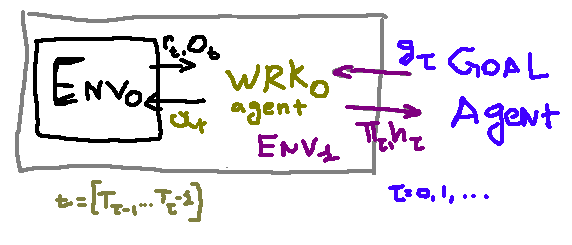
\includegraphics[width=0.9\linewidth]{./assets/ga_wrk_hierarchy.png}
  \caption{
  \emph{Layers of abstraction (encapsulation)}:
  the goalsetter treats the worker in its environment jointly as a single
  black-box (non-diff'able with internal time-scale $t$) environment with
  states $h_\tau$, rewards $pi_\tau$ and goals $g_\tau$ as control.
  % 
  \attn{crude sketch. MAYBE an ``onion'' with the goalsetter at the core?}
  }
  \label{fig:environment_hierarchy}
\end{figure}


\section{Additional reviews}

To review: \citep{guo_self-imitation_2019}, \citep{liu_learning_2018} -- looks like path rl,
and, of course, \citep{citation_needed}.

\medskip

% this should be rewrtitten, as it does not answer any review question:
%  contributions, relevance, criticism
A triplet of papers \citep{hafner_learning_2019,hafner_dream_2020,hafner_mastering_2020} propose
to learn the optimal control policy via dynamics in the latent space, wherein a stochastic
model of the world is identified and the agent learns its policy using the analytical
gradients through the learnt dynamics and reward function.
%
In \citep[alg.~1]{hafner_dream_2020} the training alternates between learning latent dynamics
and observation-to-latent representations, and optimizing the policy in the latent space of
the \emph{virtual} environment determined by the identified ``world model''.
% iterative learning control
The world model is trained from experience and the policy is trained with a frozen world model.

During the second phase experience is collected in the real environment (how?)
% act out the learnt policy in the real env through the representation model.

The model of the ground-truth environment is that of the partially observed MDP (incomplete
information) with the following
\begin{align*}
  a_t & \sim p(a \mid o_{\leq t}, a_{< t})
    \,, \\
  o_{t+1}, r_{t+1}
    & \sim p_t(o, r \mid o_{\leq t}, a_{< t}, a_t)
    \,,
\end{align*}
where non-stationarity of $p_t$ is due to the unobserved true full state of the environment.
% 
The proposed world model is
\begin{equation*}
  \begin{aligned}
    & \text{representation model}
      & & h_{t+1} \sim p(h \mid h_t, a_{\leq t}, o_{\leq t})
          \,, \\
    & \text{transition dynamics}
      & & h_{t+1} \sim q(h \mid h_t, a_t)
          \,, \\
    & \text{rewards}
      & & r_{t+1} \sim q(r \mid h_{t+1})
          \,, \\
  \end{aligned}
\end{equation*}
and the agent's policy (and value for actor-critic) depends on the inferred latent state $
  a_t \sim \pi(a\mid h_t)
$. The model is designed in such way that it is possible to differentiably sample from it.

The policy is learnt using the imagined trajectories cast from the current state of the 
ground-truth environment: infer the recent latent state $h_t$ from the history $
  (o_s, a_s, r_s)_{s \leq t}
$ and ``dream'' latent differentiable trajectories from it $
  (h_\tau, a_\tau, r_\tau)_{\tau \geq t}
$ with $a_\tau \sim \pi(a\mid h_\tau)$ and the transition and reward dynamics. The agent
maximizes $
  \mathbb{E}_{\pi}^{\geq t} \bigl\{
      \sum_{s \geq \tau} \gamma^{s - \tau} r_s
    \bigr\}
$ using path derivatives rather than score-function approach.
% 
Since we backprop through a recurrent system, the we face the issue of exploding, of
vanishing gradients, if the largest-magnitude of eigenvalue of the latent-to-latent
Jacobian is not away from the the unit circle.

It might be useful to treat this as sort of ``seq-to-seq'' training where we learn
a policy $\pi$ on the latent state to maximize the sequence of returns or Generalized
Advantage Estimates, \citep{schulman_high-dimensional_2016}. Since reducing the while
future trajectory since $\tau$ just to as single return $G_\tau$ might result in poor
credit assignment.

The imaginary world model is trained using the ELBO \attn{what variational approximations?}.
\footnote{
  The inference engines $q$ as opposed to models $p(O, A)$, with the former approximating
  the model-based posterior.
}
%
The policy is parameterized by
$$
a = \tanh\Bigl(\mathcal{N}\bigl(
    \mu(h), \operatorname{diag}{\sigma^2(h)}
  \bigr)\Bigr)
  \,. $$


\citet{chen_decision_2021} appeal to the upside-down RL paradigm and treat the task as
a large seq-to-seq learning task. The most interesting piece is conditioning the action
taken on the desired return from taking the action and following some generalized policy
later on.

% XXX what is a plan? can we create ``options'' on-the-fly and enrich the action space
%  with them? DO we need specia lagos for this, or the PPO, A2C of the good'ol DQN could
%  do the trick? ?

\section{What is this?}

\paragraph{What is this?} % (fold)
\label{par:what_is_this}

This has been copied from some old notebook of mine that had no context. It appears to be
related to PPO, \citep{schulman_proximal_2017}, and ENAS.
%
Policy-gradient (non-rigorous):
$$
L^\text{PG}(\theta)
    := \hat{\mathbb{E}}_t
        \log \pi(a_t\mid s_t; \theta) \widehat{A}_t
    \,. $$
Importance weight for old-vs-current policy
$$
w_t(\theta)
    := \frac{\pi(a_t \mid s_t; \theta)}{\pi(a_t \mid s_t; \theta_-)}
\,. $$
TRPO (non-rigorous):
$$
\begin{aligned}
    &\underset{\theta}{\text{maximum}}
      & &
        \hat{\mathbb{E}}_t w_t(\theta) \widehat{A}_t
        \,, \\
    & \text{subject to}
      & & \hat{\mathbb{E}}_t
        \operatorname{KL}\bigl(
            \pi(\cdot \mid s_t; \theta)
            \| \pi(\cdot \mid s_t; \theta_-)
        \bigr) \leq \delta
    \,.
\end{aligned}
    $$
But constrained optimization is ``hard'' in TRPO, so PPO uses the regularized objective.
% 
The current policy loss
$$
L(\theta)
    := \hat{\mathbb{E}}_t w_t(\theta) \widehat{A}_t
    \,. $$
The clipped-ratio policy loss
$$
L^\text{CLIP}(\theta)
    := \hat{\mathbb{E}}_t \min\bigl\{
        w_t(\theta) \widehat{A}_t,
        \operatorname{clip}(w_t(\theta), 1 - \varepsilon, 1 + \varepsilon) \widehat{A}_t
    \bigr\}
    \,, $$
where $\operatorname{clip}$ removes the incentive for moving $w_t(\theta)$ away from one,
and $\min$ makes the objective into a lower bound on $L(\theta)$.

Policy loss with KL-penalty
$$
L^\text{KLPEN}(\theta)
    := L^\text{CLIP}(\theta)
    - \beta \, \hat{\mathbb{E}}_t
        \operatorname{KL}\bigl(
            \pi(a \mid s_t, \theta_-)
            \| \pi(a \mid s_t, \theta)
        \bigr)
    \,, $$
uses adaptive regulator for $\beta$ when the Kullback-Leibler divergence ``exceeds''
($\times 2$ if $> d_\text{trg} \frac32$) or ``undershoots'' the target ($\div 2$
if $< d_\text{trg} \frac23$).

Negative to what is computed in \texttt{PPO.policy\_loss}
\begin{align}
\max_\theta L^\text{enas}(\theta)
    &= L^\text{CLIP}(\theta)
        + (\mathrm{entropy\_coef})\, \hat{\mathbb{E}}_t \mathbb{H}(\pi(a_t\mid s_t, \theta))
    \\
        &+ \beta \underbrace{
            \mathbb{E}_{a\sim \pi(a \mid s_t, \theta_-)} \log \pi(a \mid s_t, \theta)
        }_{\text{what is left of KL}}
    \,.
\end{align}
Everywhere $\hat{\mathbb{E}}_t$ is average over the sample $
    S_t = (a_{ti}, s_{ti}, \widehat{A}_{ti})_{i=1}^m
$.

% paragraph what_is_this (end)    


\end{document}
